\section{Why we evaluate models}


\begin{frame}{Why evaluate a model?}
    \begin{itemize}
        \item The goal of supervised learning is to predict well on \emph{new} observations $(\mathbf{x}^\ast, y^\ast)$, not on the data used for fitting
        \item Error on the fitting (training) data is an over-optimistic estimate of error on new data
        \item We need honest estimates of performance on data the model has not seen
        \item Two related tasks:
        \begin{itemize}
            \item \textbf{Model assessment}: how well does the final model perform?
            \item \textbf{Model selection}: which model, or which level of flexibility, should we choose?
        \end{itemize}
    \end{itemize}
\end{frame}


\begin{frame}{Training error vs. test error}
    \begin{itemize}
        \item Regression, with $n$ training observations:
    \end{itemize}
    \[
        \mathrm{MSE}_{\text{train}} = \frac{1}{n}\sum_{i=1}^{n}\big(y^{(i)} - \hat{f}(\mathbf{x}^{(i)})\big)^2,
        \qquad
        \mathrm{MSE}_{\text{test}} = \mathbb{E}\big[(y^\ast - \hat{f}(\mathbf{x}^\ast))^2\big]
    \]
    \begin{itemize}
        \item $\mathrm{MSE}_{\text{test}}$ is estimated on a held-out set $\mathcal{T}$ of $m$ observations: $\frac{1}{m}\sum_{i\in\mathcal{T}}\big(y^{(i)} - \hat{f}(\mathbf{x}^{(i)})\big)^2$
        \item Classification: error rate $\frac{1}{n}\sum_{i=1}^{n} I\big(y^{(i)} \neq \hat{y}^{(i)}\big)$, with the test version defined analogously
        \item Fitting methods minimize training error, so a small training error does \emph{not} guarantee a small test error
    \end{itemize}
\end{frame}


\section{Overfitting and underfitting}


\begin{frame}{Underfitting and overfitting}
    \begin{itemize}
        \item \textbf{Underfitting}: the model is too simple to capture the structure in $f$
        \begin{itemize}
            \item High error on the training data \emph{and} on the test data
        \end{itemize}
        \item \textbf{Overfitting}: the model is so flexible that it fits the noise $\epsilon$ in the training sample
        \begin{itemize}
            \item Very low training error, but much higher test error
        \end{itemize}
        \item Diagnosis: compare training and test (or validation) error
        \begin{itemize}
            \item Both high $\Rightarrow$ underfitting; large gap between them $\Rightarrow$ overfitting
        \end{itemize}
    \end{itemize}
\end{frame}



\begin{frame}{Example: polynomial fits to simulated data}
    \begin{figure}
        \centering
        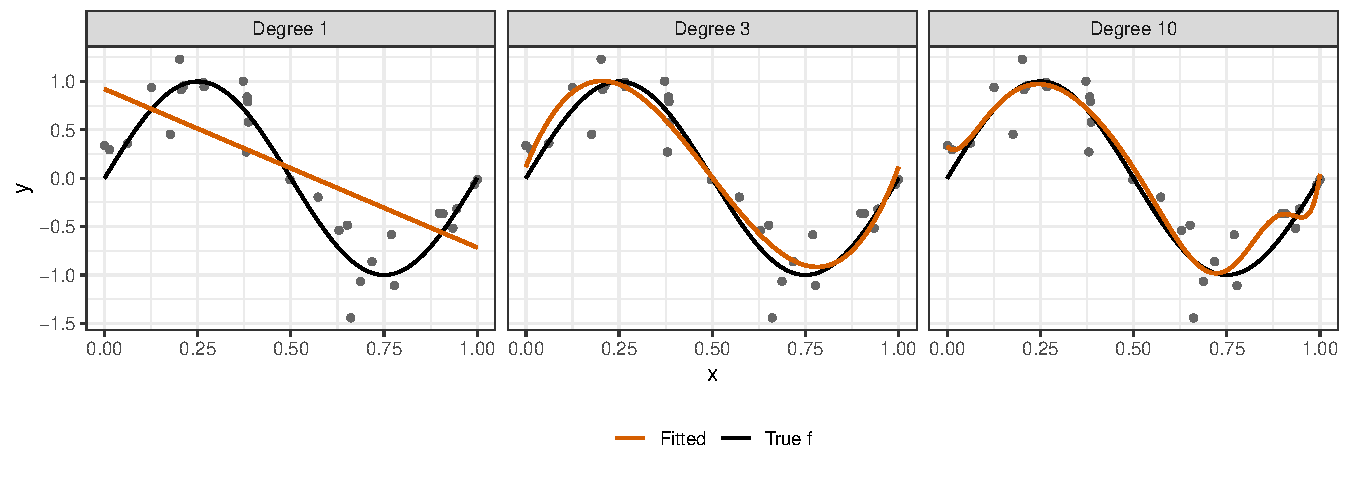
\includegraphics[width=\linewidth]{figures/sim_fits.pdf}
    \end{figure}
    \begin{itemize}
        \item Data: $y = \sin(2\pi x) + \epsilon$ with $\epsilon \sim N(0, 0.3^2)$ and $n = 30$; fits are polynomials of degree 1, 3 and 10
        \item Degree 1 underfits; degree 3 is close to the truth; degree 10 chases the noise
    \end{itemize}
\end{frame}


\begin{frame}{Training error vs. test error as flexibility grows}
    \begin{columns}[T]
        \begin{column}{0.55\textwidth}
            \begin{figure}
                \centering
                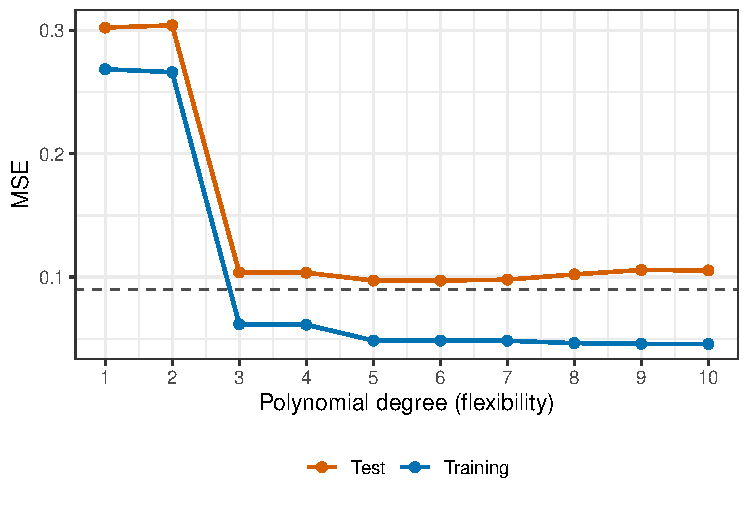
\includegraphics[width=\linewidth]{figures/sim_train_test_mse.pdf}
            \end{figure}
        \end{column}
        \begin{column}{0.43\textwidth}
            \begin{itemize}
                \item Training MSE decreases as the degree increases
                \item Test MSE is U-shaped: it first falls, then rises
                \item The dashed line is $\sigma^2$, the error no model can beat
                \item Choosing the model with the smallest training MSE would select the most overfit model
            \end{itemize}
        \end{column}
    \end{columns}
\end{frame}


\begin{frame}{What to do about under- and overfitting}
    \begin{columns}[T]
        \begin{column}{0.48\textwidth}
            \textbf{If underfitting}
            \begin{itemize}
                \item Use a more flexible model
                \item Add features or interactions
                \item Reduce regularization
            \end{itemize}
        \end{column}
        \begin{column}{0.48\textwidth}
            \textbf{If overfitting}
            \begin{itemize}
                \item Use a simpler model
                \item Collect more training data
                \item Remove features or add regularization
            \end{itemize}
        \end{column}
    \end{columns}
    \svspace{1em}
    \begin{itemize}
        \item Both remedies move the model along the flexibility axis; finding the right point requires an honest estimate of test error
    \end{itemize}
\end{frame}


\section{The bias-variance trade-off}


\begin{frame}{Bias-variance decomposition: setup}
    \begin{itemize}
        \item Assume $y^\ast = f(\mathbf{x}^\ast) + \epsilon$ with $\mathbb{E}[\epsilon] = 0$, $\mathrm{Var}(\epsilon) = \sigma^2$, and $\epsilon$ independent of the training data
        \item The estimate $\hat{f}$ is computed from a random training set $\mathcal{D}$, so $\hat{f}(\mathbf{x}^\ast)$ is itself a random variable
        \item Expected test MSE at a fixed point $\mathbf{x}^\ast$, taken over training sets $\mathcal{D}$ and noise $\epsilon$:
    \end{itemize}
    \[
        \mathbb{E}\big[(y^\ast - \hat{f}(\mathbf{x}^\ast))^2\big]
    \]
    \begin{itemize}
        \item Goal: split this quantity into interpretable pieces
    \end{itemize}
\end{frame}


\begin{frame}{Bias-variance decomposition: step 1 (noise)}
    Substitute $y^\ast = f(\mathbf{x}^\ast) + \epsilon$ and expand the square (writing $f$ and $\hat{f}$ for $f(\mathbf{x}^\ast)$ and $\hat{f}(\mathbf{x}^\ast)$):
    \begin{align*}
        \mathbb{E}\big[(y^\ast - \hat{f})^2\big]
            &= \mathbb{E}\big[(f - \hat{f} + \epsilon)^2\big] \\
            &= \mathbb{E}\big[(f - \hat{f})^2\big] + 2\,\mathbb{E}\big[\epsilon\,(f - \hat{f})\big] + \mathbb{E}[\epsilon^2]
    \end{align*}
    \begin{itemize}
        \item $\epsilon$ is independent of $\hat{f}$ and has mean zero, so the cross term is $2\,\mathbb{E}[\epsilon]\,\mathbb{E}[f - \hat{f}] = 0$
        \item $\mathbb{E}[\epsilon^2] = \mathrm{Var}(\epsilon) = \sigma^2$
    \end{itemize}
    \[
        \mathbb{E}\big[(y^\ast - \hat{f})^2\big] = \mathbb{E}\big[(f - \hat{f})^2\big] + \sigma^2
    \]
    \dual{}{The same argument applies at every $\mathbf{x}^\ast$; averaging over the distribution of $\mathbf{x}^\ast$ gives the overall expected test MSE.}
\end{frame}

\begin{frame}{Bias-variance decomposition: step 2 (bias and variance)}
    Let $\bar{f} = \mathbb{E}[\hat{f}(\mathbf{x}^\ast)]$. Add and subtract $\bar{f}$ inside the remaining term:
    \begin{align*}
        \mathbb{E}\big[(f - \hat{f})^2\big]
            &= \mathbb{E}\big[\big((f - \bar{f}) + (\bar{f} - \hat{f})\big)^2\big] \\
            &= (f - \bar{f})^2 + 2\,(f - \bar{f})\,\mathbb{E}\big[\bar{f} - \hat{f}\big] + \mathbb{E}\big[(\bar{f} - \hat{f})^2\big]
    \end{align*}
    \begin{itemize}
        \item $f - \bar{f}$ is a constant and $\mathbb{E}[\bar{f} - \hat{f}] = 0$, so the cross term vanishes
    \end{itemize}
    \[
        \mathbb{E}\big[(y^\ast - \hat{f}(\mathbf{x}^\ast))^2\big]
        = \underbrace{\mathrm{Var}\big(\hat{f}(\mathbf{x}^\ast)\big)}_{\text{variance}}
        + \underbrace{\big[\mathrm{Bias}\big(\hat{f}(\mathbf{x}^\ast)\big)\big]^2}_{\text{squared bias}}
        + \underbrace{\sigma^2}_{\text{irreducible}}
    \]
    with $\mathrm{Bias}(\hat{f}(\mathbf{x}^\ast)) = \mathbb{E}[\hat{f}(\mathbf{x}^\ast)] - f(\mathbf{x}^\ast)$.
\end{frame}

\begin{frame}{Interpreting the three terms}
    \begin{itemize}
        \item \textbf{Variance}: how much $\hat{f}(\mathbf{x}^\ast)$ changes if we refit on a different training set
        \begin{itemize}
            \item Flexible methods follow the training sample closely, so their variance is high
        \end{itemize}
        \item \textbf{Bias}: error from approximating the true $f$ by a simpler model class
        \begin{itemize}
            \item A straight line fitted to a curved $f$ is wrong on average, however much data we have
        \end{itemize}
        \item \textbf{Irreducible error} $\sigma^2$: noise in $y^\ast$; a lower bound on test MSE
        \item More flexibility typically lowers bias and raises variance; the test MSE depends on which changes faster
    \end{itemize}
\end{frame}


\begin{frame}{The trade-off in simulation}
    \begin{columns}[T]
        \begin{column}{0.55\textwidth}
            \begin{figure}
                \centering
                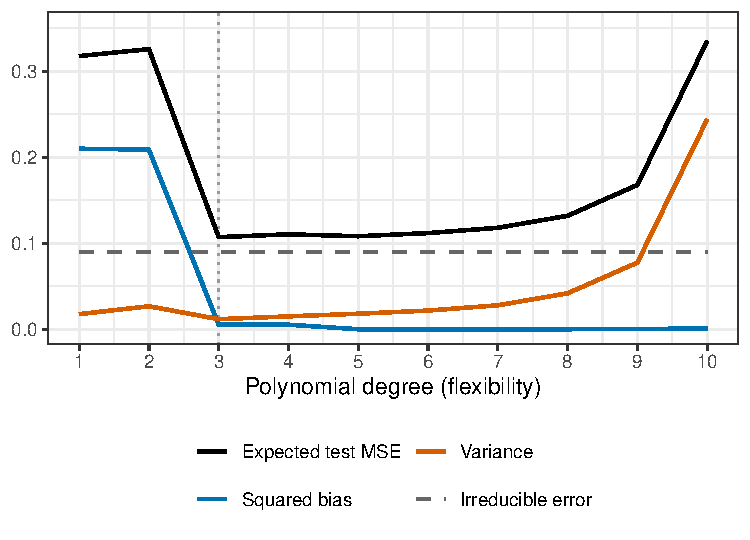
\includegraphics[width=\linewidth]{figures/sim_biasvar_decomp.pdf}
            \end{figure}
        \end{column}
        \begin{column}{0.43\textwidth}
            \begin{itemize}
                \item Estimated from 500 simulated training sets, averaged over $x^\ast \in [0,1]$
                \item Squared bias falls and variance rises with the polynomial degree
                \item Expected test MSE is their sum plus $\sigma^2$
                \item The best degree depends on $f$, $n$ and $\sigma^2$; more data moves the optimum towards more flexible models
            \end{itemize}
        \end{column}
    \end{columns}
\end{frame}


\begin{frame}{Bias-variance for classification}
    \begin{sitemize}
        \item With the 0--1 loss the decomposition is not additive in the simple form above, but the same qualitative behaviour holds.
        \item Flexible classifiers have low bias and high variance, while rigid ones have the reverse.
        \item The test error rate is again U-shaped in flexibility, so it must be estimated without using the training error.
    \end{sitemize}
\end{frame}


\section{Validation set and cross-validation}


\begin{frame}{Running example: mpg vs. horsepower (\texttt{Auto})}
    \begin{columns}[T]
        \begin{column}{0.55\textwidth}
            \begin{figure}
                \centering
                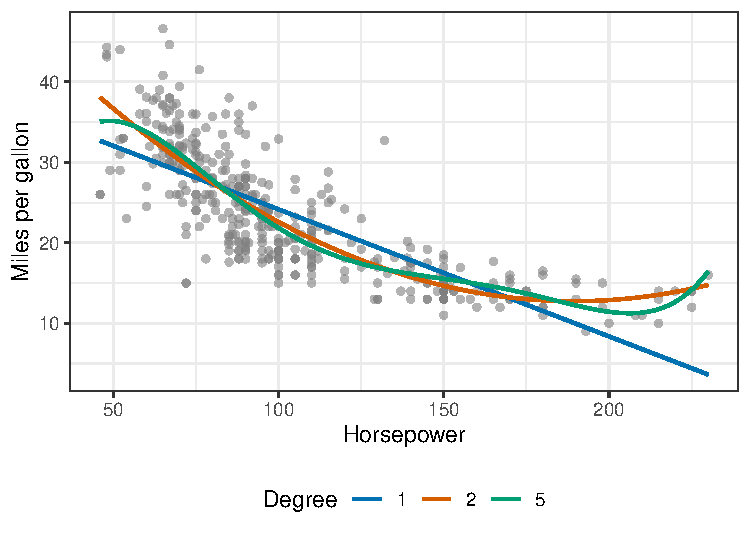
\includegraphics[width=\linewidth]{figures/auto_fits.pdf}
            \end{figure}
        \end{column}
        \begin{column}{0.43\textwidth}
            \begin{itemize}
                \item $n = 392$ cars; response mpg, predictor horsepower
                \item Model: polynomial regression $\hat{f}(x) = \hat{\beta}_0 + \hat{\beta}_1 x + \dots + \hat{\beta}_d x^d$
                \item The degree $d$ controls flexibility; which $d$ should we use?
            \end{itemize}
        \end{column}
    \end{columns}
\end{frame}


\begin{frame}{Training, validation and test sets}
    \begin{center}
        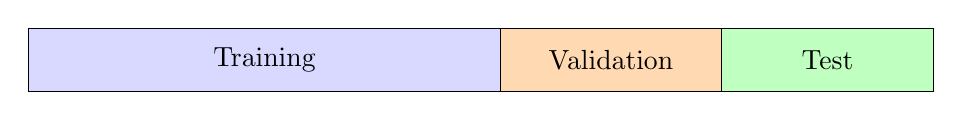
\begin{tikzpicture}
            \draw[fill=blue!15]   (0,0)   rectangle (6,0.8)   node[midway] {Training};
            \draw[fill=orange!30] (6,0)   rectangle (8.8,0.8) node[midway] {Validation};
            \draw[fill=green!25]  (8.8,0) rectangle (11.5,0.8) node[midway] {Test};
        \end{tikzpicture}
    \end{center}
    \begin{itemize}
        \item \textbf{Training set}: used to fit the parameters of each candidate model
        \item \textbf{Validation set}: used to compare candidates and tune flexibility
        \item \textbf{Test set}: used once, at the end, to assess the chosen model; never used for any choice
        \item If test data influence any decision, the test error is no longer an honest estimate
    \end{itemize}
\end{frame}


\begin{frame}{Validation set approach}
    \begin{figure}
        \centering
        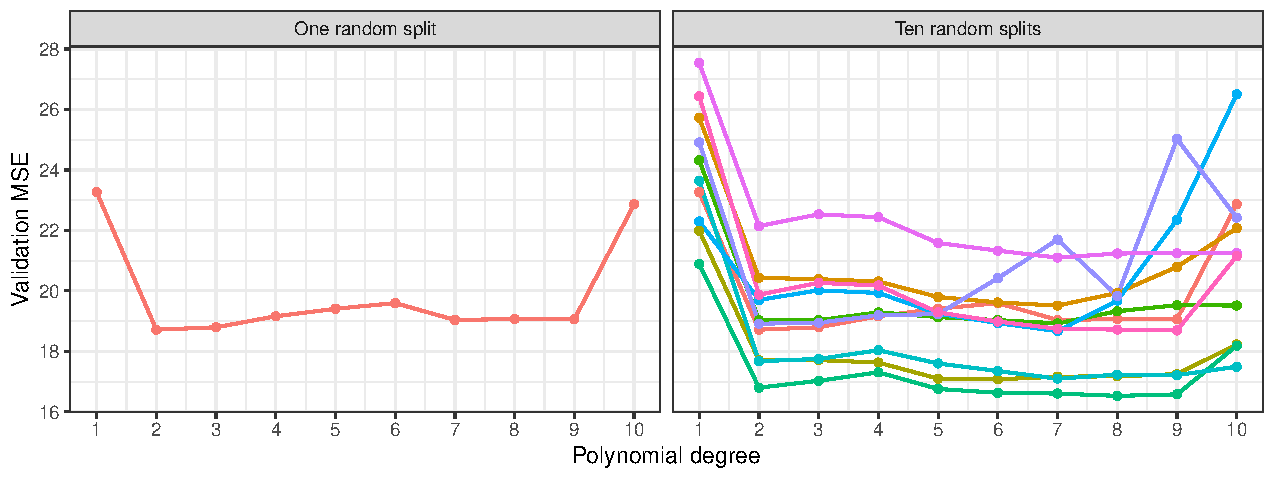
\includegraphics[width=0.92\linewidth]{figures/auto_validation_splits.pdf}
    \end{figure}
    \begin{itemize}
        \item Randomly split the data into two halves; fit on one, compute the MSE on the other
        \item The estimate, and even the best degree, changes from split to split (right panel)
        \item Only part of the data is used for fitting, so the validation MSE tends to overestimate the test MSE
    \end{itemize}
\end{frame}

\begin{frame}{Leave-one-out cross-validation (LOOCV)}
    \begin{itemize}
        \item Hold out observation $i$, fit on the remaining $n-1$, predict $y^{(i)}$; repeat for $i = 1, \dots, n$
    \end{itemize}
    \[
        \mathrm{CV}_{(n)} = \frac{1}{n}\sum_{i=1}^{n}\mathrm{MSE}_i,
        \qquad
        \mathrm{MSE}_i = \big(y^{(i)} - \hat{y}^{(i)}_{(-i)}\big)^2
    \]
    \begin{itemize}
        \item $\hat{y}^{(i)}_{(-i)}$ is the prediction for $\mathbf{x}^{(i)}$ from the model fitted without observation $i$
        \item Each fit uses $n-1$ points, so the bias of the estimate is small, and there is no randomness in the splits
        \item For least squares with hat values $h_i$, one fit suffices:
    \end{itemize}
    \[
        \mathrm{CV}_{(n)} = \frac{1}{n}\sum_{i=1}^{n}\left(\frac{y^{(i)} - \hat{y}^{(i)}}{1 - h_i}\right)^2
    \]
\end{frame}


\begin{frame}{$k$-fold cross-validation}
    \begin{columns}[T]
        \begin{column}{0.5\textwidth}
            \begin{center}
                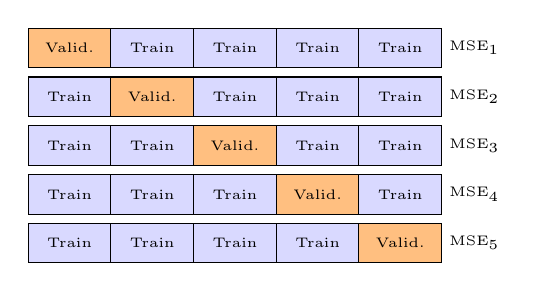
\begin{tikzpicture}[fold/.style={draw, minimum width=1.05cm, minimum height=0.5cm, font=\tiny}]
                    \foreach \j in {1,...,5} {
                        \foreach \i in {1,...,5} {
                            \ifnum\i=\j
                                \node[fold, fill=orange!50] at (\i*1.05, -\j*0.62) {Valid.};
                            \else
                                \node[fold, fill=blue!15] at (\i*1.05, -\j*0.62) {Train};
                            \fi
                        }
                        \node[font=\tiny, anchor=west] at (5.75, -\j*0.62) {$\mathrm{MSE}_{\j}$};
                    }
                \end{tikzpicture}
            \end{center}
        \end{column}
        \begin{column}{0.48\textwidth}
            \begin{itemize}
                \item Randomly partition the data into $k$ folds $F_1, \dots, F_k$ of about equal size ($k = 5$ shown)
                \item For each $j$: fit on all folds except $F_j$, evaluate on $F_j$
            \end{itemize}
        \end{column}
    \end{columns}
    \[
        \mathrm{MSE}_j = \frac{1}{|F_j|}\sum_{i \in F_j}\big(y^{(i)} - \hat{f}^{(-j)}(\mathbf{x}^{(i)})\big)^2,
        \qquad
        \mathrm{CV}_{(k)} = \frac{1}{k}\sum_{j=1}^{k}\mathrm{MSE}_j
    \]
\end{frame}


\begin{frame}{Validation set, LOOCV and $k$-fold compared}
    \begin{center}
        \small
        \begin{tabular}{lccc}
            \toprule
            Method & Model fits & Bias of estimate & Variance of estimate \\
            \midrule
            Validation set & 1 & high & high \\
            LOOCV ($k = n$) & $n$ & lowest & high \\
            $k$-fold ($k = 5, 10$) & $k$ & low to moderate & moderate \\
            \bottomrule
        \end{tabular}
    \end{center}
    \begin{itemize}
        \item LOOCV training sets are nearly identical, so its $n$ fitted models are highly correlated and their average has high variance
        \item Smaller $k$ means more bias (less training data per fit) but less variance and less computation
        \item Empirically, $k = 5$ or $k = 10$ gives estimates that suffer neither from excessive bias nor from high variance
    \end{itemize}
\end{frame}


\begin{frame}{Cross-validation on \texttt{Auto}}
    \begin{figure}
        \centering
        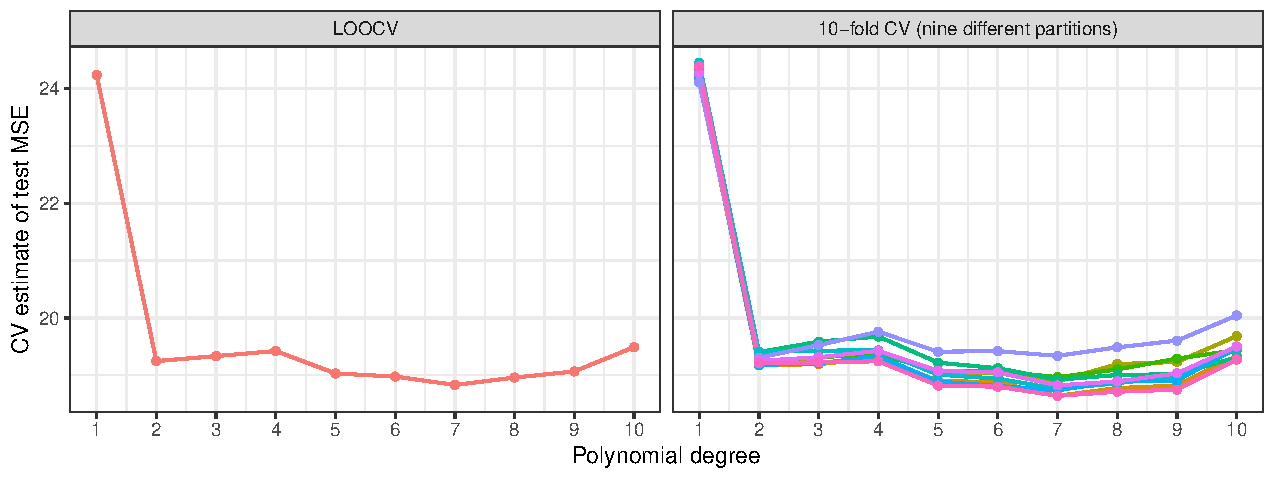
\includegraphics[width=0.92\linewidth]{figures/auto_cv_curves.pdf}
    \end{figure}
    \begin{itemize}
        \item CV error drops from about 24.2 (linear) to about 19.2 (quadratic), with no clear gain beyond degree 2
        \item Ten-fold CV curves from different random partitions agree closely, unlike the validation set curves
        \item The location of the minimum matters more than the exact level of the estimate
    \end{itemize}
\end{frame}

\begin{frame}{Cross-validation for classification}
    \begin{itemize}
        \item Replace the squared error by the misclassification indicator
    \end{itemize}
    \[
        \mathrm{Err}_j = \frac{1}{|F_j|}\sum_{i\in F_j} I\big(y^{(i)} \neq \hat{y}^{(i)}\big),
        \qquad
        \mathrm{CV}_{(k)} = \frac{1}{k}\sum_{j=1}^{k}\mathrm{Err}_j
    \]
    \begin{itemize}
        \item Any other metric (precision, recall, AUC, \dots) can be computed per fold and averaged in the same way
    \end{itemize}
\end{frame}


\section{Classification metrics}


\begin{frame}{The confusion matrix}
    \begin{columns}[T]
        \begin{column}{0.5\textwidth}
            \begin{center}
                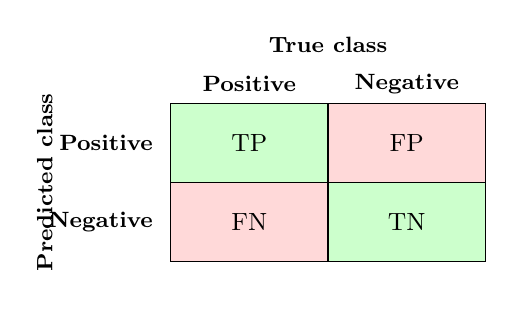
\begin{tikzpicture}[
                        cell/.style={draw, minimum width=2.0cm, minimum height=1.0cm, align=center, font=\small},
                        lab/.style={font=\footnotesize\bfseries, align=center}
                    ]
                    \node[cell, fill=green!20] at (0,0)      {TP};
                    \node[cell, fill=red!15]   at (2.0,0)    {FP};
                    \node[cell, fill=red!15]   at (0,-1.0)   {FN};
                    \node[cell, fill=green!20] at (2.0,-1.0) {TN};
                    \node[lab] at (0,0.75)     {Positive};
                    \node[lab] at (2.0,0.75)   {Negative};
                    \node[lab] at (1.0,1.25)   {True class};
                    \node[lab, anchor=east] at (-1.1,0)    {Positive};
                    \node[lab, anchor=east] at (-1.1,-1.0) {Negative};
                    \node[lab, rotate=90] at (-2.6,-0.5)   {Predicted class};
                \end{tikzpicture}
            \end{center}
        \end{column}
        \begin{column}{0.48\textwidth}
            \begin{itemize}
                \item Rows: predicted class; columns: true class (the layout used in ISLP; some software transposes it)
                \item TP, TN: correct predictions; FP (false alarm), FN (miss): errors
                \item The positive class is the one we care about detecting
                \item For $K > 2$ classes the matrix is $K \times K$
            \end{itemize}
        \end{column}
    \end{columns}
\end{frame}


\begin{frame}{Example: \texttt{Default} data, threshold 0.5}
    \begin{columns}[T]
        \begin{column}{0.5\textwidth}
            \begin{center}
                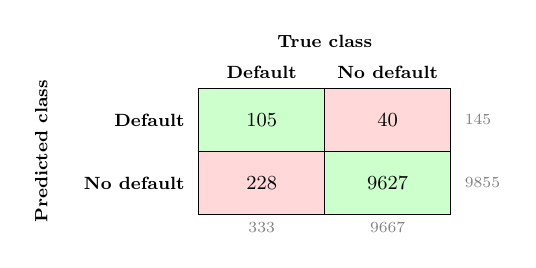
\begin{tikzpicture}[scale=0.8, every node/.append style={transform shape},
                        cell/.style={draw, minimum width=2.0cm, minimum height=1.0cm, align=center, font=\small},
                        lab/.style={font=\footnotesize\bfseries, align=center},
                        tot/.style={font=\scriptsize, gray}
                    ]
                    \node[cell, fill=green!20] at (0,0)      {105};
                    \node[cell, fill=red!15]   at (2.0,0)    {40};
                    \node[cell, fill=red!15]   at (0,-1.0)   {228};
                    \node[cell, fill=green!20] at (2.0,-1.0) {9627};
                    \node[lab] at (0,0.75)     {Default};
                    \node[lab] at (2.0,0.75)   {No default};
                    \node[lab] at (1.0,1.25)   {True class};
                    \node[lab, anchor=east] at (-1.1,0)    {Default};
                    \node[lab, anchor=east] at (-1.1,-1.0) {No default};
                    \node[lab, rotate=90] at (-3.5,-0.5)   {Predicted class};
                    \node[tot] at (0,-1.7)   {333};
                    \node[tot] at (2.0,-1.7) {9667};
                    \node[tot, anchor=west] at (3.1,0)    {145};
                    \node[tot, anchor=west] at (3.1,-1.0) {9855};
                \end{tikzpicture}
            \end{center}
        \end{column}
        \begin{column}{0.48\textwidth}
            \begin{itemize}
                \item Logistic regression of \texttt{default} on \texttt{student}, \texttt{balance}, \texttt{income}; $n = 10{,}000$ with 333 defaulters
                \item Predict ``default'' when $\hat{p}(\mathbf{x}^\ast) > 0.5$
                \item Matrix computed on the training data, as in ISLP; on new data expect somewhat worse numbers
            \end{itemize}
        \end{column}
    \end{columns}
\end{frame}


\begin{frame}{Accuracy and error rate}
    \[
        \text{Accuracy} = \frac{TP + TN}{TP + FP + FN + TN},
        \qquad
        \text{Error rate} = 1 - \text{Accuracy}
    \]
    \begin{itemize}
        \item \texttt{Default}: accuracy $= (105 + 9627)/10000 = 97.3\%$
        \item A classifier that always predicts ``no default'' has accuracy $9667/10000 = 96.7\%$ while catching no defaulter at all
        \item With imbalanced classes, accuracy mostly measures how large the majority class is
        \item Use accuracy when classes are roughly balanced and both error types cost about the same
    \end{itemize}
\end{frame}


\begin{frame}{Precision, recall and specificity}
    \begin{align*}
        \text{Precision} &= \frac{TP}{TP + FP}
            && \text{flagged cases that are truly positive} \\
        \text{Recall (sensitivity)} &= \frac{TP}{TP + FN}
            && \text{true positives that we find} \\
        \text{Specificity} &= \frac{TN}{TN + FP}
            && \text{true negatives that we clear}
    \end{align*}
    \begin{itemize}
        \item \texttt{Default} at threshold 0.5: precision $= 105/145 \approx 0.72$, recall $= 105/333 \approx 0.32$, specificity $= 9627/9667 \approx 0.996$
        \item High accuracy and high specificity hide that two thirds of the defaulters are missed
        \item False positive rate $= FP/(FP + TN) = 1 - \text{specificity}$
    \end{itemize}
\end{frame}


\begin{frame}{Precision vs. recall: intuition}
    \begin{columns}[T]
        \begin{column}{0.48\textwidth}
            \textbf{Precision:} ``When I raise an alarm, how often am I right?''
            \begin{itemize}
                \item Spam filter: a real email sent to the spam folder is costly, a few spam emails in the inbox are not
                \item Fraud alerts reviewed by a small team: every false alert wastes investigator time
            \end{itemize}
        \end{column}
        \begin{column}{0.48\textwidth}
            \textbf{Recall:} ``Of all real cases, how many did I catch?''
            \begin{itemize}
                \item Cancer screening: a missed case is far worse than an extra follow-up test
                \item Flood or earthquake early warning: a missed event is catastrophic, a false alarm is an inconvenience
            \end{itemize}
        \end{column}
    \end{columns}
    \svspace{1em}
    \begin{itemize}
        \item Targeting cash transfers to poor households: low recall excludes eligible households, low precision leaks money to the non-poor
        \item Specificity matters when clearing negatives is the goal, e.g.\ avoiding unnecessary treatment
    \end{itemize}
\end{frame}


\begin{frame}{Which metric should I use?}
    \begin{center}
        \small
        \begin{tabular}{p{5.6cm}p{5.0cm}}
            \toprule
            Situation & Metric to emphasize \\
            \midrule
            Balanced classes, similar error costs & Accuracy \\
            False positives are costly & Precision, specificity \\
            False negatives are costly & Recall (sensitivity) \\
            Rare positives, both errors matter & $F_1$ score, precision--recall curve \\
            Comparing classifiers over all thresholds & ROC curve and AUC \\
            \bottomrule
        \end{tabular}
    \end{center}
    \begin{itemize}
        \item Decide which error is more expensive \emph{before} looking at the numbers
        \item Always compare against a trivial baseline such as the majority-class classifier
    \end{itemize}
\end{frame}


\begin{frame}{Changing the threshold}
    \begin{itemize}
        \item Classify as positive when $\hat{p}(\mathbf{x}^\ast) > \tau$; lowering $\tau$ flags more cases
    \end{itemize}
    \begin{center}
        \footnotesize
        \begin{tabular}{rrrrrrrrr}
            \toprule
            $\tau$ & TP & FP & FN & TN & Accuracy & Precision & Recall & $F_1$ \\
            \midrule
            0.5 & 105 &  40 & 228 & 9627 & 0.973 & 0.724 & 0.315 & 0.439 \\
            0.2 & 203 & 277 & 130 & 9390 & 0.959 & 0.423 & 0.610 & 0.499 \\
            0.1 & 248 & 560 &  85 & 9107 & 0.936 & 0.307 & 0.745 & 0.435 \\
            \bottomrule
        \end{tabular}
    \end{center}
    \begin{itemize}
        \item Recall rises as $\tau$ falls, while precision and accuracy fall: the two error types trade off
        \item The right $\tau$ depends on the relative costs of missing a defaulter and of rejecting a good customer
    \end{itemize}
\end{frame}


\begin{frame}{Metrics as a function of the threshold}
    \begin{figure}
        \centering
        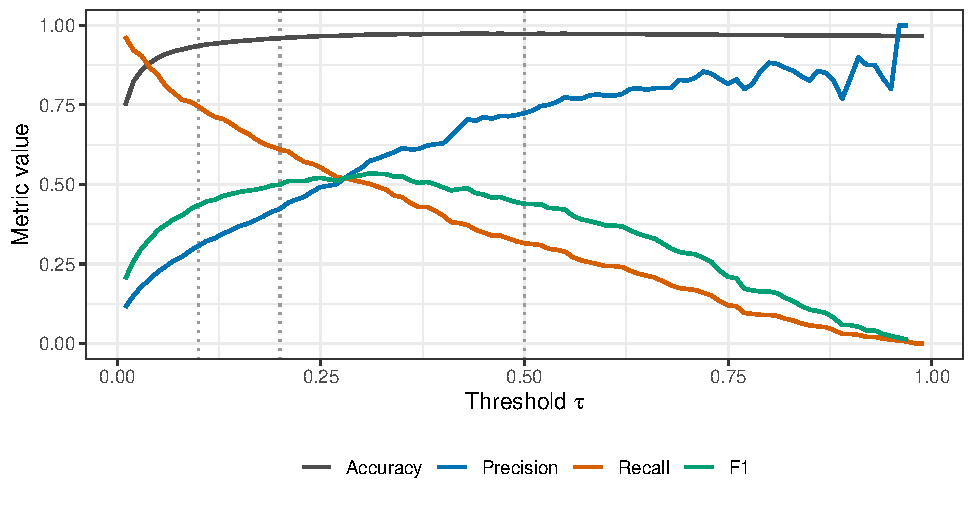
\includegraphics[width=0.75\linewidth]{figures/default_threshold_metrics.pdf}
    \end{figure}
    \begin{itemize}
        \item Recall decreases monotonically in $\tau$; precision tends to increase, but not monotonically
        \item Accuracy is highest at large $\tau$ simply because most cases are negative
    \end{itemize}
\end{frame}

\begin{frame}{The $F_1$ score}
    \[
        F_1 = \frac{2\cdot\text{Precision}\cdot\text{Recall}}{\text{Precision} + \text{Recall}} = \frac{2\,TP}{2\,TP + FP + FN}
    \]
    \begin{itemize}
        \item Harmonic mean of precision and recall: it is low unless \emph{both} are reasonably high
        \item Ignores $TN$, so it is not inflated by a large negative class
        \item $F_\beta = (1 + \beta^2)\,\dfrac{\text{Precision}\cdot\text{Recall}}{\beta^2\,\text{Precision} + \text{Recall}}$ weights recall $\beta$ times as much as precision
        \item For $K > 2$ classes, compute the metric per class and average (macro-average), or pool the counts (micro-average)
    \end{itemize}
\end{frame}


\begin{frame}{ROC curve, precision--recall curve and AUC}
    \begin{figure}
        \centering
        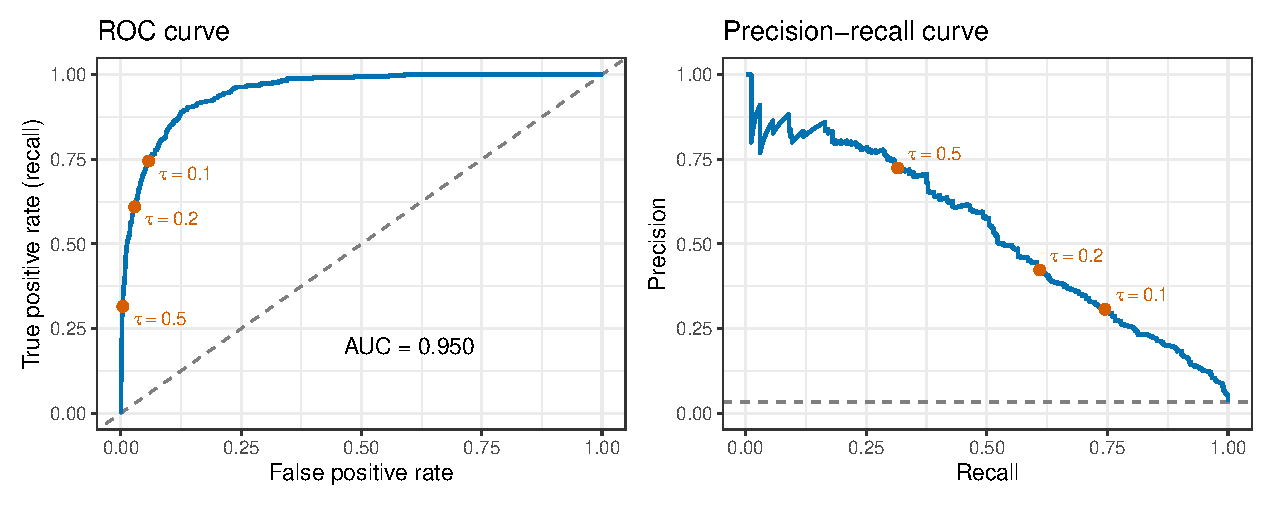
\includegraphics[width=0.92\linewidth]{figures/default_roc_pr.pdf}
    \end{figure}
    \begin{itemize}
        \item ROC: true positive rate (recall) against false positive rate as $\tau$ varies; AUC $\approx 0.95$ here (training data)
        \item AUC is the probability that a random positive receives a higher $\hat{p}$ than a random negative; 0.5 is chance, 1 is perfect
        \item With rare positives the precision--recall curve is more informative; its chance level is the prevalence (about 3.3\%)
    \end{itemize}
\end{frame}


\section{Model selection and comparison}


\begin{frame}{A workflow for selection and assessment}
    \begin{enumerate}
        \item Split off a test set and set it aside
        \item On the training data, use CV to compare candidate models and to tune hyperparameters such as the polynomial degree
        \item Refit the chosen model on the entire training set
        \item Evaluate it once on the test set and report that number
    \end{enumerate}
    \begin{itemize}
        \item The CV error of the winning model is optimistic, because it was selected for having the lowest CV error
    \end{itemize}
\end{frame}


\begin{frame}{Adjusted $R^2$, AIC and BIC}
    \begin{itemize}
        \item Penalize the training fit for model size instead of using held-out data; $d$ = number of predictors, $p$ = number of estimated parameters
    \end{itemize}
    \[
        R^2_{\text{adj}} = 1 - \frac{\mathrm{RSS}/(n - d - 1)}{\mathrm{TSS}/(n - 1)},
        \qquad
        \mathrm{AIC} = -2\log\hat{L} + 2p,
        \qquad
        \mathrm{BIC} = -2\log\hat{L} + p\log n
    \]
    \begin{center}
        \mode<presentation>{\small}
        \begin{tabular}{crrr}
            \toprule
            Degree & $R^2_{\text{adj}}$ & AIC & BIC \\
            \midrule
            1 & 0.605 & 2363.3 & 2375.2 \\
            2 & 0.686 & 2274.4 & \textbf{2290.2} \\
            3 & 0.686 & 2275.5 & 2295.4 \\
            4 & 0.686 & 2276.1 & 2299.9 \\
            5 & 0.693 & 2268.7 & 2296.5 \\
            6 & \textbf{0.695} & \textbf{2266.7} & 2298.4 \\
            \bottomrule
        \end{tabular}
    \end{center}
\end{frame}


\begin{frame}{Adjusted $R^2$, AIC, BIC or cross-validation?}
    \begin{itemize}
        \item Lower AIC and BIC are better; higher $R^2_{\text{adj}}$ is better
        \item BIC has the heavier penalty ($\log n > 2$ for $n \geq 8$) and picks the quadratic; AIC and $R^2_{\text{adj}}$ favour a higher degree
        \item These criteria assume a likelihood-based model and a well-defined parameter count, and they rely on the training fit
        \item CV assumes little about the model and works for any method and any metric, at the cost of refitting the model several times
    \end{itemize}
\end{frame}


\begin{frame}{Comparing models fairly}
    \begin{itemize}
        \item Compare all models on exactly the same folds, so that differences are not due to different splits
        \item Use the metric that matches the goal (MSE, recall, $F_1$, AUC, \dots), and include a trivial baseline
        \item Look at per-fold differences between two models and their standard error, not just the two means
        \item A small difference relative to the SE is not evidence that one model is better
        \item Report the final performance on the untouched test set
    \end{itemize}
\end{frame}


\begin{frame}{Summary}
    \begin{itemize}
        \item Training error is optimistic; estimate test error with held-out data
        \item Test error is U-shaped in flexibility: $\mathbb{E}[(y^\ast - \hat{f}(\mathbf{x}^\ast))^2] = \mathrm{Var} + \mathrm{Bias}^2 + \sigma^2$
        \item $k$-fold CV ($k = 5$ or $10$) is the default tool for model assessment and selection
        \item Classification: read the confusion matrix, then choose accuracy, precision, recall, $F_1$ or AUC according to the costs of the two error types
        \item Select with CV (or AIC/BIC) on the training data, and touch the test set only once
    \end{itemize}
\end{frame}